% =========================================================================
%  Auditing Generalization Claims for LLM Agent Harnesses (Phase-7C / v5)
%  Official ICLR 2027 style (media.iclr.cc/Conferences/ICLR2027/iclr-2027-style-files.zip)
% =========================================================================
\documentclass{article}
\usepackage{iclr2027_conference,times}
\usepackage{hyperref}
\hypersetup{hidelinks}
\usepackage{url}
\usepackage{microtype}
\usepackage{booktabs}
\usepackage{longtable}
\usepackage{array}
\usepackage{amsmath}\usepackage{amssymb}\usepackage{pifont}
\usepackage{enumitem}
\setlist{nosep,leftmargin=1.3em,topsep=2pt,parsep=0pt,itemsep=1pt}
\usepackage{tikz}\usetikzlibrary{shapes.geometric,arrows.meta,positioning}

\title{Auditing Generalization Claims for LLM Agent Harnesses:\\Semantic Binding and Measurement Validity}

\author{Anonymous Authors\\ Paper submitted for double-blind review}

%\iclrfinalcopy

\begin{document}
\maketitle

\begin{abstract}
We introduce a \emph{claim-scope framework} for evaluating harness interventions in LLM agents, separating four progressively stronger generalization claims---local effect, within-family held-out confirmation, cross-model transfer, and cross-family transfer---and showing that evidence at one level does not imply the next. On a controlled tool-grounded \emph{semantic-handoff} task, a non-answer-bearing ``clarity bundle'' (BundleS) suppresses a specific tool-green semantic-binding failure for Qwen3.7-Max (Level~0) and survives a pre-frozen held-out instance (Level~1). Under exact counterbalancing the effect is not established for DeepSeek-V4-Pro (Level~2); cross-family transfer is likewise not established (Level~3): a prospective twelve-instance expansion reversed the descriptive direction relative to a three-instance pilot without establishing a treatment effect, while a second family sits at a non-discriminative ceiling. We introduce a second, orthogonal axis---a four-layer \emph{Harness Effect Audit Protocol} (capability, sampling, execution, artifact integrity)---and show that each layer caught a concrete threat that would have changed the scientific conclusion. An external taxonomy scope probe (Terminal-Bench 2.0$\to$2.1, 26 repairs) shows the taxonomy has external relevance but incomplete coverage (1 direct, 21 partial, 4 outside; sampling layer 0). Our controlled task instances test existence, recurrence, and transfer direction rather than estimate population-level pass rates.
\end{abstract}

% ========================================================================
\section{Introduction}
% ========================================================================
When a harness intervention changes agent behavior, what can we claim? We introduce a \textbf{claim-scope ladder} with four levels and show that surviving one level does not imply surviving the next:

\begin{itemize}
\item \textbf{Level~0 (local effect):} a harness intervention changes behavior for a model within a controlled task family.
\item \textbf{Level~1 (within-family confirmation):} the effect survives a pre-frozen held-out instance from the same semantic/generator family.
\item \textbf{Level~2 (cross-model transfer):} the effect survives under a different model backend with matched task semantics.
\item \textbf{Level~3 (cross-family transfer):} the effect survives on independently constructed semantic task families.
\end{itemize}
\textbf{Evidence at level $k$ does not imply evidence at level $k+1$.} Failure at a higher level does \emph{not} refute the lower-level effect; it bounds the claim's scope.

Our frozen evidence maps to the ladder as follows: Level~0 (Qwen3.7-Max workflow Base 1/3 $\to$ BundleS 3/3), Level~1 (pre-frozen held-out: 1/3 $\to$ 3/3), Level~2 (DeepSeek-V4-Pro: 3/4 = 3/4, not established), Level~3 (prospective STA $n$=12: not established; SPICE: ceiling/non-discriminative).

A harness-effect claim has two independent questions: (A)~\emph{what scope of generalization does the evidence support?} and (B)~\emph{was the measurement itself valid?} The claim-scope ladder addresses (A); a four-layer audit protocol (capability, sampling, execution, artifact integrity) addresses (B). Figure~\ref{fig:2d} places our concrete evidence and incidents into this 2D framework.

\paragraph{Contributions.} (1)~A claim-scope framework separating local effects, within-family confirmation, cross-model transfer, and cross-family transfer, with the principle that each level requires independent evidence. (2)~A controlled semantic-binding study showing a real local/within-family effect but no established higher-level transfer, including a prospective 12-instance expansion whose descriptive direction reversed relative to a 3-instance pilot. (3)~A measurement-validity framework showing how capability, sampling, execution, and artifact failures materially changed scientific interpretation. (4)~Supporting external taxonomy evidence from Terminal-Bench repairs.

% ========================================================================
\section{Related Work and Problem Formulation}
% ========================================================================
\paragraph{Harnesses and harness effects.} A \emph{harness} is the task-level information structure visible to the agent (prompt, visible files, disclosure bundle, public tool feedback, action surface). A \emph{harness effect} is a change in semantic-binding correctness attributable to harness information content, holding the hidden truth, grader, and tool fixed.

\paragraph{Problem formulation.} Each task is a \emph{semantic handoff}: bind a tuple to canonical typed roles from role-misleading evidence. The workflow family binds PVT descriptors to typed axes; Family~A (STA/PrimeTime) binds (intent\_class, target\_partition, check\_mode) from an authority provenance DAG; Family~B (SPICE/HSPICE) binds (corner, load\_condition, metric) from a request--authority join.

\paragraph{TAB vs.\ semantic binding.} Task alignment~\citep{tab} asks \emph{which} environmental evidence an agent should follow; semantic binding asks \emph{which semantic role} selected evidence is permitted to fill. Our failures can occur after relevant evidence has been retrieved and can remain tool-green---the agent finds the right artifact but binds its value to the wrong typed axis.

\paragraph{Positioning.} \citet{harnessbench} broadly characterize model$\times$harness interactions; \citet{harnesseval} critique harness-leaderboard conflation; \citet{harnesso} optimize harnesses; \citet{abc} and \citet{protocolval} address benchmark-construction and protocol-validity standards. We differ by introducing a claim-scope ladder, isolating a controlled semantic-binding mechanism, and auditing which measurement failures changed the scientific conclusion (Table~\ref{tab:novelty}). \citet{longhorizon} report cross-benchmark harness gains, which we use as evidence that some interventions do transfer---so transfer must be demonstrated rather than assumed. Concurrently, \citet{harnessaudit} audits trajectory-level safety properties of harness execution (boundary compliance, execution fidelity, system stability; 210 tasks across 8 domains); our object differs---we audit the evidentiary scope and measurement validity of semantic-binding performance claims, not execution-trajectory safety.

\begin{table}[h]
\centering\small
\caption{Positioning relative to related work.}
\label{tab:novelty}
\begin{tabular}{p{0.20\linewidth} p{0.36\linewidth} p{0.36\linewidth}}
\toprule
Prior work & What it establishes & What this paper additionally does \\
\midrule
Harness-Bench~\citep{harnessbench} & Broad model$\times$harness characterization & Claim-scope ladder + controlled semantic mechanism \\
Rethinking~\citep{harnesseval} & Leaderboard conflation; search/overfitting & Level $k$ need not imply level $k{+}1$ \\
HarnessOpt-Bench~\citep{harnesso} & Optimizer capability & Studies validity of harness-effect claims \\
ABC~\citep{abc} / Protocol validity~\citep{protocolval} & Setup; shortcut/reward validity & Per-control threat log \\
\bottomrule
\end{tabular}
\end{table}

% ========================================================================
\section{Methodology: The 2D Framework}
% ========================================================================
\paragraph{The claim-scope ladder ($x$-axis).} Any harness-effect claim lives at one of four levels (Level~0--3 above). Moving right on the ladder requires evidence at the new level; passing a lower level is necessary but not sufficient.

\paragraph{The measurement-validity axis ($y$-axis).} Any measurement has four independent validity layers: (1)~capability validity (does the task measure the intended capability, including tool-green semantic alternatives?); (2)~sampling validity (repeated trajectories, counterbalancing, membership arbitration); (3)~execution validity (transport, terminal-vs-recovered, tool health, protocol completion); (4)~artifact integrity (action-surface isolation, canonical-source integrity, custody).

\begin{figure}[h]
\centering\footnotesize
\caption{The 2D framework: claim scope ($x$) $\times$ measurement validity ($y$). Rows are the four measurement-validity layers (capability, sampling, execution, artifact integrity). Each cell lists the study's concrete evidence or incident.}
\label{fig:2d}
\begin{tabular}{p{0.10\linewidth}|p{0.20\linewidth} p{0.20\linewidth} p{0.20\linewidth} p{0.20\linewidth}}
\toprule
 & \textbf{Local} & \textbf{Within-family} & \textbf{Cross-model} & \textbf{Cross-family} \\
\midrule
\textbf{Cap.} & tool-green wrong binding; typed oracle & held-out: BundleS 3/3 & DeepSeek 3/4=3/4 & STA $n$=12 not established; SPICE ceiling \\
\textbf{Samp.} & position-balanced blocking; non-det. & pre-frozen held-out inst. & counterbalanced block & prospective 12-inst. schedule \\
\textbf{Exec.} & SSE streaming (censoring caught) & recovered degradation kept & --- & SPICE action-surface repair \\
\textbf{Art.} & canonical-tree guard & custody hashes & --- & --- \\
\bottomrule
\end{tabular}
\end{figure}

\paragraph{Construct: what semantic correctness means.}
Semantic correctness is \emph{not} inferred from tool success, a hidden numeric answer, or the artifact score. It is decided solely by whether the submitted tuple matches the binding attested by the independent provenance/authority oracle. \emph{Worked example (Family~A):} visible evidence attests intent=\emph{functional\_close}, partition=\emph{core}, check\_mode=\emph{setup}; the agent submits (functional\_close, core, \emph{both})---PrimeTime returns green, the value is type-valid, but the coverage authority attests \emph{setup}, not \emph{both}; the oracle rejects it as a role-conditioned value-selection failure. This construct is instantiated independently in the workflow family (PVT axes), Family~A (intent/partition/check\_mode), and Family~B (corner/load/metric), each with its own grader. We do \emph{not} claim human validation (Study~B was preregistered but unexecuted).

\paragraph{Conditions.} \textbf{Base} (ambiguous handoff; no answer-bearing disclosure); \textbf{BundleS} (canonical labels, value-domain definitions, glossary, procedural contract; no answer-bearing C6; no golden values); \textbf{TypedContract} (same information as BundleS as a JSON Schema). Hidden truth and grader are identical across conditions.

\paragraph{Design and models.} Seeded exact-counterbalanced blocked randomization, frozen before any paid call. Instance is the primary unit; repetitions nested. We evaluate Qwen3.7-Max and DeepSeek-V4-Pro; these are not representative of the frontier-model population. The design is diagnostic, not population-estimating: it tests existence, recurrence, ceiling/null behavior, and transfer direction; it cannot resolve small effect sizes.

% ========================================================================
\section{Study I --- Local and Within-Family Effect (RQ1; Levels 0--1)}
% ========================================================================
On the workflow controlled pair (identical truth/grader; ambiguous vs.\ clear handoff), BundleS suppresses the axis-binding failure for Qwen3.7-Max: Base 1/3 (2 axis-binding) $\to$ BundleS 3/3 (0 axis-binding). The schema/contract subset (excluding answer-bearing C6) suffices on the development pair, and generalizes to a \emph{pre-frozen held-out} instance: BundleS 3/3 vs Base 1/3. The failure taxonomy (Figure~\ref{fig:taxonomy}) partitions the workflow ledger (54 episodes) into 29 correct, 20 \emph{axis-binding}, and 5 \emph{role-conditioned value-selection}---all tool-green, rejected only by the typed oracle.

A sequential decomposition tested whether a stable minimal component underlies BundleS. None was isolated: C1 alone, C2-only, C4-only, and a C24 bridge all failed their thresholds. The bundle-level effect is real within-family; the operative sub-component is not identified.

\textbf{Level~0 and Level~1 are established for Qwen3.7-Max.} We make no universal improvement claim. Failure at Level~2 or Level~3 does not refute this local/within-family effect.

\begin{figure}[h]
\centering
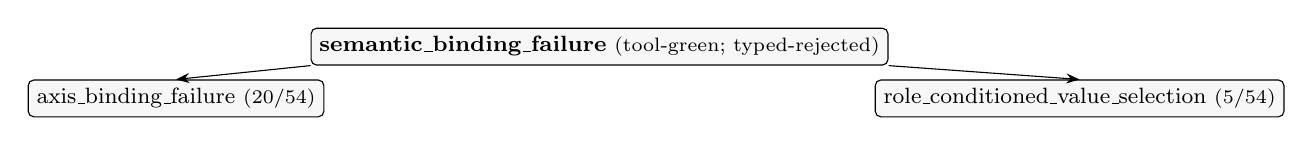
\begin{tikzpicture}[every node/.style={font=\footnotesize},
  box/.style={draw,rounded corners=2pt,inner sep=3pt,align=left,fill=gray!6}]
\node[box] (root) {\textbf{semantic\_binding\_failure} \scriptsize(tool-green; typed-rejected)};
\node[box, below left=5pt and -5pt of root] (a) {axis\_binding\_failure \scriptsize(20/54)};
\node[box, below right=5pt and -5pt of root] (v) {role\_conditioned\_value\_selection \scriptsize(5/54)};
\draw[-{Stealth}] (root.south west) -- (a.north); \draw[-{Stealth}] (root.south east) -- (v.north);
\end{tikzpicture}
\caption{Semantic-binding failure taxonomy.}
\label{fig:taxonomy}
\end{figure}

% ========================================================================
\section{Study II --- Cross-Model and Cross-Family Transfer (RQ2; Levels 2--3)}
% ========================================================================
\textit{Does the Level~0--1 effect transfer?} Table~\ref{tab:main} is the main result.

\begin{table}[h]
\centering\small
\caption{Main result matrix (semantic-binding correctness; instance is the unit). Workflow/SPICE entries are correct of $k$ stochastic repetitions; STA entries are the mean correct-rate over 12 instances.}
\label{tab:main}
\begin{tabular}{p{0.30\linewidth} c c c c l}
\toprule
Family / model & Base & BundleS & TypedContract & \#inst. & verdict \\
\midrule
Workflow / Qwen3.7-Max (Level~0) & 1/3 & 3/3 & --- & 1 & local effect \\
Workflow / Qwen3.7-Max (Level~1, held-out) & 1/3 & 3/3 & --- & 1 & within-family \\
Workflow / DeepSeek-V4-Pro (Level~2) & 3/4 & 3/4 & --- & 1 & not established \\
\textbf{STA / Qwen3.7-Max (Level~3, prospective)} & \textbf{0.208} & \textbf{0.333} & \textbf{0.458} & \textbf{12} & \textbf{not established} \\
SPICE / Qwen3.7-Max (Level~3) & 1.00 & 1.00 & 1.00 & 3 & ceiling \\
\bottomrule
\end{tabular}
\end{table}

\paragraph{Level~2 (cross-model).} Under exact counterbalancing, BundleS is not established for DeepSeek-V4-Pro (3/4 = 3/4). This does not refute the Level~0--1 effect for Qwen3.7-Max; it bounds the claim's scope.

\paragraph{Level~3 (cross-family, STA).} Across 12 pre-registered instances, BundleS vs Base: 3 improving, 2 declining, 7 tied; exact sign-test $p=1.0$; permutation sensitivity $p=0.31$. \emph{The three-instance pilot and the prospectively frozen twelve-instance batch differed even in their descriptive ordering. We interpret this as evidence that very small task panels are unreliable for directional Harness claims, not as evidence that BundleS transfers; small-panel instability of directional benchmark claims has been independently documented for agent-safety benchmarks~\citep{safetycap}.} TypedContract is descriptively highest (0.458) but no preregistered TypedContract advantage was established; this is hypothesis-generating only. The pilot ($n$=3) is not pooled with the prospective $n$=12.

\begin{table}[h]
\centering\footnotesize
\caption{Prospective STA per-instance outcomes ($n$=12; Y=correct, n=wrong).}
\label{tab:sta12}
\begin{tabular}{l ccc ccc}
\toprule & \multicolumn{3}{c}{2-rep (rate)} & \multicolumn{3}{c}{diff} \\
\cmidrule(lr){2-4}\cmidrule(lr){5-7} inst. & Base & BundleS & TC & S$-$B & TC$-$B & TC$-$S \\ \midrule
0004 & nY(.5) & nn(0) & nn(0) & $-$.5 & $-$.5 & .0 \\
0005 & nn(0) & nn(0) & nn(0) & .0 & .0 & .0 \\
0006 & nn(0) & nn(0) & nn(0) & .0 & .0 & .0 \\
0007 & Yn(.5) & nn(0) & nn(0) & $-$.5 & $-$.5 & .0 \\
0008 & nn(0) & nn(0) & nn(0) & .0 & .0 & .0 \\
0009 & nn(0) & nn(0) & nn(0) & .0 & .0 & .0 \\
0010 & nY(.5) & YY(1) & YY(1) & .5 & .5 & .0 \\
0011 & nn(0) & YY(1) & YY(1) & 1.0 & 1.0 & .0 \\
0012 & nn(0) & YY(1) & YY(1) & 1.0 & 1.0 & .0 \\
0013 & YY(1) & YY(1) & YY(1) & .0 & .0 & .0 \\
0014 & nn(0) & nn(0) & Yn(.5) & .0 & .5 & .5 \\
0015 & nn(0) & nn(0) & YY(1) & .0 & 1.0 & 1.0 \\
\bottomrule
\end{tabular}
\end{table}

\paragraph{Level~3 (cross-family, SPICE).} Base = BundleS = TypedContract = 1.00---a non-discriminative ceiling. This is a measurement limitation, not evidence against transfer.

\paragraph{Three outcomes, kept distinct.} The transfer evidence yields: (i)~\emph{no established effect on a discriminating family} (STA, $n$=12): informative but cannot rule out a small effect; (ii)~\emph{ceiling} (SPICE): Base already solves the binding; no headroom; (iii)~\emph{direction reversal under prospective expansion} (STA pilot vs.\ prospective): evidence that very small panels are unreliable for directional claims. We report each separately and do not pool.

% ========================================================================
\section{Study III --- Measurement Validity and External Scope Probe (RQ3)}
% ========================================================================
Each headline conclusion could have been manufactured or masked by a measurement artifact. The four-layer protocol is instantiated and stress-tested; Table~\ref{tab:incidents} lists incidents where a control \emph{materially changed the interpretation}.

\begin{table}[h]
\centering\footnotesize
\caption{Audit-protocol incidents: each control prevented or corrected an invalid scientific interpretation.}
\label{tab:incidents}
\begin{tabular}{p{0.26\linewidth} p{0.30\linewidth} p{0.36\linewidth}}
\toprule
Threat & Control & Conclusion that would have been wrong \\
\midrule
Non-streaming censoring (Exec) & SSE + terminal-transport arbiter & Qwen3.7-Max falsely recorded as failing \\
Position confounding (Samp) & Exact position-balanced blocking & Base/BundleS order leaked into contrast \\
Recovered degradation (Exec) & Terminal-valid vs recovered split & Hard-but-recovered solve discarded \\
PT corrupted measurement (Exec) & Tool-health sentinel + bookends & Tool hiccup read as model failure \\
SPICE action-surface false positive (Art) & Immutable core + forensic audit & 12 SPICE episodes spuriously zeroed; semantic-binding ceiling obscured \\
Canonical-source mutation (Art) & Exact-commit worktree + hash guard & Golden rewrite read as tool outage \\
\bottomrule
\end{tabular}
\end{table}

\paragraph{Why the controls materially affected interpretation.} Without SSE streaming, Qwen3.7-Max would have been recorded as failing the controlled pair---inverting RQ1. Without the SPICE action-surface repair, all twelve SPICE episodes would have been spuriously zeroed, creating an apparent score floor that obscured the true semantic-binding ceiling. Without the canonical-hash guard, a silent golden rewrite would have masqueraded as a day-long tool outage. Each would have altered the headline interpretation.

\paragraph{External taxonomy scope probe (Terminal-Bench 2.0$\to$2.1).} As an external scope probe (not validation), we coded the 26 officially documented repairs under the four-layer-plus-Other rubric, \emph{frozen before coding}: \textbf{1 direct, 21 partial, 4 outside} (of 26); layers: capability 17, sampling 0, execution 10, artifact 1; 6 multi-layer. We interpret this as evidence that the taxonomy has \emph{external relevance but incomplete coverage}. This is static retrospective taxonomy application; it does \emph{not} validate runtime portability and does \emph{not} validate every audit layer (the sampling layer received no external support). The full 26-task coding is in the Appendix.

% ========================================================================
\section{Limitations and Discussion}
% ========================================================================
\emph{Controlled executable tasks, not sampled production incidents.} \emph{EDA-heavy environments}---transfer results are scoped to EDA. \emph{Small instance counts}---Level~0 and Level~2 rest on $n$=1; the design is diagnostic, not population-estimating. \emph{Construct validity}---rests on executable provenance/authority oracles; the preregistered human construct-validity study (Study~B) is preregistered but unexecuted; we do not claim human validation. \emph{Model scope}---two models, not representative of the frontier population. \emph{Audit protocol}---instantiated and stress-tested here, not broadly validated; the external probe shows relevance but incomplete coverage. \emph{No mechanism isolated}---the bundle-level effect is real within-family but no stable minimal component was identified.

\paragraph{Discussion.} The claim-scope ladder makes generalization claims auditable: a reader can locate any harness-effect claim at a specific level and ask whether the evidence supports it. The measurement-validity axis makes the measurement independently checkable. Together they answer: \emph{what scope does the evidence support, and was the measurement itself valid?} Some harness interventions do transfer~\citep{longhorizon}; transfer is therefore an empirical property that must be demonstrated, not assumed.

\paragraph{Reproducibility.} Deterministic generators (fixed seeds); independent per-family graders; exact-commit isolated-worktree execution with pre/post-episode canonical-hash verification; committed sample-membership arbitration; validity-only replacement; per-episode custody byte-matching. Program totals: 58+24+36+72 paid primary episodes; committed-ledger cost \textyen{}745.29.

% ========================================================================
\section{Conclusion}
% ========================================================================
We introduced a claim-scope framework for harness-effect generalization claims and showed that a local/within-family effect (Levels~0--1) did not establish cross-model (Level~2) or cross-family (Level~3) transfer. A prospective 12-instance expansion reversed the descriptive direction while still not establishing a treatment effect. The measurement-validity framework showed that capability, sampling, execution, and artifact controls each materially changed the scientific conclusion. The contribution is a framework for auditing what evidence supports a generalization claim---not a proposal of an improved harness.

\bibliographystyle{iclr2027_conference}
\bibliography{references}

% ========================================================================
\appendix
\section{Study I --- per-instance ledger and minimal-component ablation}
Workflow ledger (54 episodes): 29 correct, 20 axis-binding, 5 role-conditioned value-selection. Minimal-component ablation (exploratory): no stable sub-component isolated (C1 alone, C2-only, C4-only, C24 bridge all failed thresholds).

\section{Study II --- prospective STA detail}
The per-instance table (Table~\ref{tab:sta12}) appears in the main text. Historical pilot ($n$=3) not pooled.

\paragraph{Statistical procedure (frozen; descriptive sensitivity only).} The task instance ($n$=12) is the independent unit; two repetitions are nested observations (72 trajectories are \emph{not} treated as $n$=72). Pilot instances 0001--0003 are excluded from the primary contrast. Each per-instance, per-condition rate is the mean over its two repetitions. The primary contrast is the signed per-instance difference $d_i = \mathrm{BundleS}_i - \mathrm{Base}_i$.
\emph{Exact paired sign test.} Of the 12 instance differences, 5 are non-zero (3 positive, 2 negative; 7 ties), so the test is conditioned on $n{=}5$ non-zero differences with $k{=}3$ positive; the two-sided exact $p$-value is $2\sum_{i=0}^{\min(k,n-k)}\binom{n}{i}/2^{n}=1.0$, excluding ties (standard convention). This is a non-establishment result, not evidence of a zero effect.
\emph{Per-instance permutation sensitivity.} Under the sharp null of no condition effect, we reshuffle the six within-instance condition labels (2 Base, 2 BundleS, 2 TypedContract) independently per instance, recompute $\sum_i(\mathrm{BundleS}_i-\mathrm{Base}_i)$, and report the two-sided proportion of $10^{4}$ Monte-Carlo replicates (fixed seed 20260811) whose absolute re-randomized sum meets or exceeds the observed $\sum_i d_i = 1.5$, giving $p=0.31$. This is a descriptive sensitivity check over the fixed instance set, \emph{not} a population-rate $p$-value (the instances are not sampled from a defined population). No adaptive $k$ was used; no trajectory-pooled $p$-value is reported; results are reported at the preregistered analysis.

\section{Study III --- full 26-task Terminal-Bench repair coding}
Rubric frozen before coding; source: PR~\#53 ``Terminal-Bench 2.1'' (body sha256 \texttt{c7172fc6}; files sha256 \texttt{fccf2d61}); 2.0/2.1 snapshots frozen (89 tasks each; sha256 \texttt{5c7ed05c}).

\begin{longtable}{p{0.27\linewidth} p{0.18\linewidth} p{0.32\linewidth} p{0.11\linewidth}}
\toprule Task & threat & mechanism & coverage \\ \midrule
adaptive-rejection-sampler & Cap & instruction clarification & partial \\
build-pmars & Cap & instruction clarification; verifier/test tightening & partial \\
caffe-cifar-10 & Exec; Cap & timeout; verifier/test broadening; instruction; env/dep; resource & partial \\
compile-compcert & Exec & environment/dependency repair & partial \\
configure-git-webserver & Cap & oracle repair; verifier/test tightening & partial \\
extract-moves-from-video & Exec & external-dependency removal & partial \\
filter-js-from-html & Cap; Exec & instruction clarification; resource increase & partial \\
fix-git & Art & hidden-artifact removal; verifier/test tightening & direct \\
hf-model-inference & Cap & verifier/test broadening & partial \\
install-windows-3.11 & Cap & instruction clarification; verifier/test tightening & partial \\
make-doom-for-mips & Exec & oracle repair; env/dep repair & partial \\
mteb-leaderboard & Exec; Cap & env/dep; instruction; resource & partial \\
mteb-retrieve & Exec; Cap & env/dep; instruction clarification & partial \\
polyglot-c-py & Cap & verifier/test broadening & partial \\
polyglot-rust-c & Cap & verifier/test broadening & partial \\
protein-assembly & Cap & oracle repair & partial \\
rstan-to-pystan & Cap & oracle repair & partial \\
sam-cell-seg & Cap & instruction clarification & partial \\
torch-tensor-parallelism & Cap; Exec & instruction clarification; resource increase & partial \\
torch-pipeline-parallelism & Exec & resource increase & partial \\
query-optimize & Cap & instruction clarification & partial \\
train-fasttext & Exec; Cap & verifier/test tightening; env/dep repair & partial \\
build-pov-ray & Other & env/dep repair & not-covered \\
financial-document-processor & Other & env/dep repair & not-covered \\
mcmc-sampling-stan & Other & env/dep repair & not-covered \\
overfull-hbox & Other & env/dep repair & not-covered \\
\bottomrule
\end{longtable}
\textbf{Aggregate:} direct 1 / partial 21 / not-covered 4; Cap 17, Exec 10, Art 1, Other 4; Samp 0; 6 multi-layer.

\section{Operational independence and phase chronology}
Five pre-registered structural criteria (independent templates, vocabularies, truths, graders, decoys). Historical chronology (provenance; does not structure the main paper): discovery $\to$ transport repair $\to$ controlled pair $\to$ held-out $\to$ cross-model $\to$ cross-family $\to$ TypedContract $\to$ prospective STA. Episodes 58/24/36/72; costs \textyen{}682.25 / \textyen{}7.72 / \textyen{}11.75 / \textyen{}43.56.

\section{Infrastructure + custody}
Exact-commit worktree; canonical-hash guard (\texttt{FAILED\_INTEGRITY} stop); episode arbiter; SSE streaming; tool-health sentinel; immutable-core/derived-deck repair; per-episode custody byte-matching. Pre-flight caught a grading-path bug (malformed signoff JSON) before the prospective run; historical pilot unaffected (0/30 triggers).

\vspace{6pt}\hrule\vspace{4pt}
\noindent\textbf{Ethics statement.} The preregistered blinded human construct-validity study (Study~B) is preregistered but unexecuted because qualified independent human annotators were unavailable; no LLM annotator was substituted.

\noindent\textbf{AI-use statement (outside the page limit).} Generative-AI assistants were used to support experimental design and critique, orchestration and infrastructure code, task generators, analysis and report scripts, literature search, result-interpretation checks, and manuscript drafting and editing. All experimental decisions, task definitions, acceptance criteria, statistical analyses, and scientific claims were reviewed and approved by the authors. Experimental results were produced by frozen executable pipelines and independently checkable graders reproduced from frozen manifests; generative-AI systems were not used as ground-truth judges or scientific oracles. The authors take responsibility for all content and conclusions.

\noindent\textbf{Reproducibility statement.} Deterministic generators, independent graders, frozen manifests, schedules, custody hashes, and sanitized episode evidence are in the anonymized supplement. ICLR 2027 deadlines: abstract September 18, 2026 AOE; full paper September 25, 2026 AOE.

\end{document}
